\documentclass[main.tex]{subfiles}
\begin{document}

\section{By-law Script}

By-law Script is a programming language with a JavaScript-like syntax specifically designed for use with the DARC protocol. Users can use By-law Script to execute a variety of tasks, including:

\begin{itemize}
    \item Operations: Users have the capability to initiate a series of operations using By-law Script. These operations encompass actions like minting and burning new tokens, token transfers, token purchases, enabling or disabling plugins, and fund withdrawals, among others.

    \item Plugin Design: By-law Script allows users to design plugins with binary expression trees, incorporating logical operators and DARC judgment expressions with parameters. These plugins can define a return type and, when necessary, specify a voting rule.

    \item Voting: By-law Script facilitates the process of voting for the current operation.
\end{itemize}

The syntax of the By-law Script closely resembles that of vanilla JavaScript, encompassing variables, constants, assignments, basic data types, functions, classes, and various other features. In addition to the fundamental JavaScript syntax, the By-law Script also supports operator overloading, which is particularly useful for describing condition nodes for plugins.

Figure 1 illustrates how the By-law Script is executed within the DARC protocol. On the operator client side, the program of the By-law Script needs to be transpiled into vanilla JavaScript. Subsequently, it is executed in the local JavaScript runtime using a code generator. After the entire program is generated within the JSON body, it takes the form of a list of operations with opcodes and parameter lists. At this point, the program is ready to be submitted from the client side as a function call to the DARC Application Binary Interface (ABI) on the EVM-compatible blockchain.

To execute the program within the DARC protocol, the DARC Software Development Kit (SDK) gains access to the address of the DARC smart contract and initiates the execution process by calling the entrance function with a wallet signature. This communication is facilitated through the JSON RPC server of the EVM-compatible blockchain.

\begin{figure}
\centering
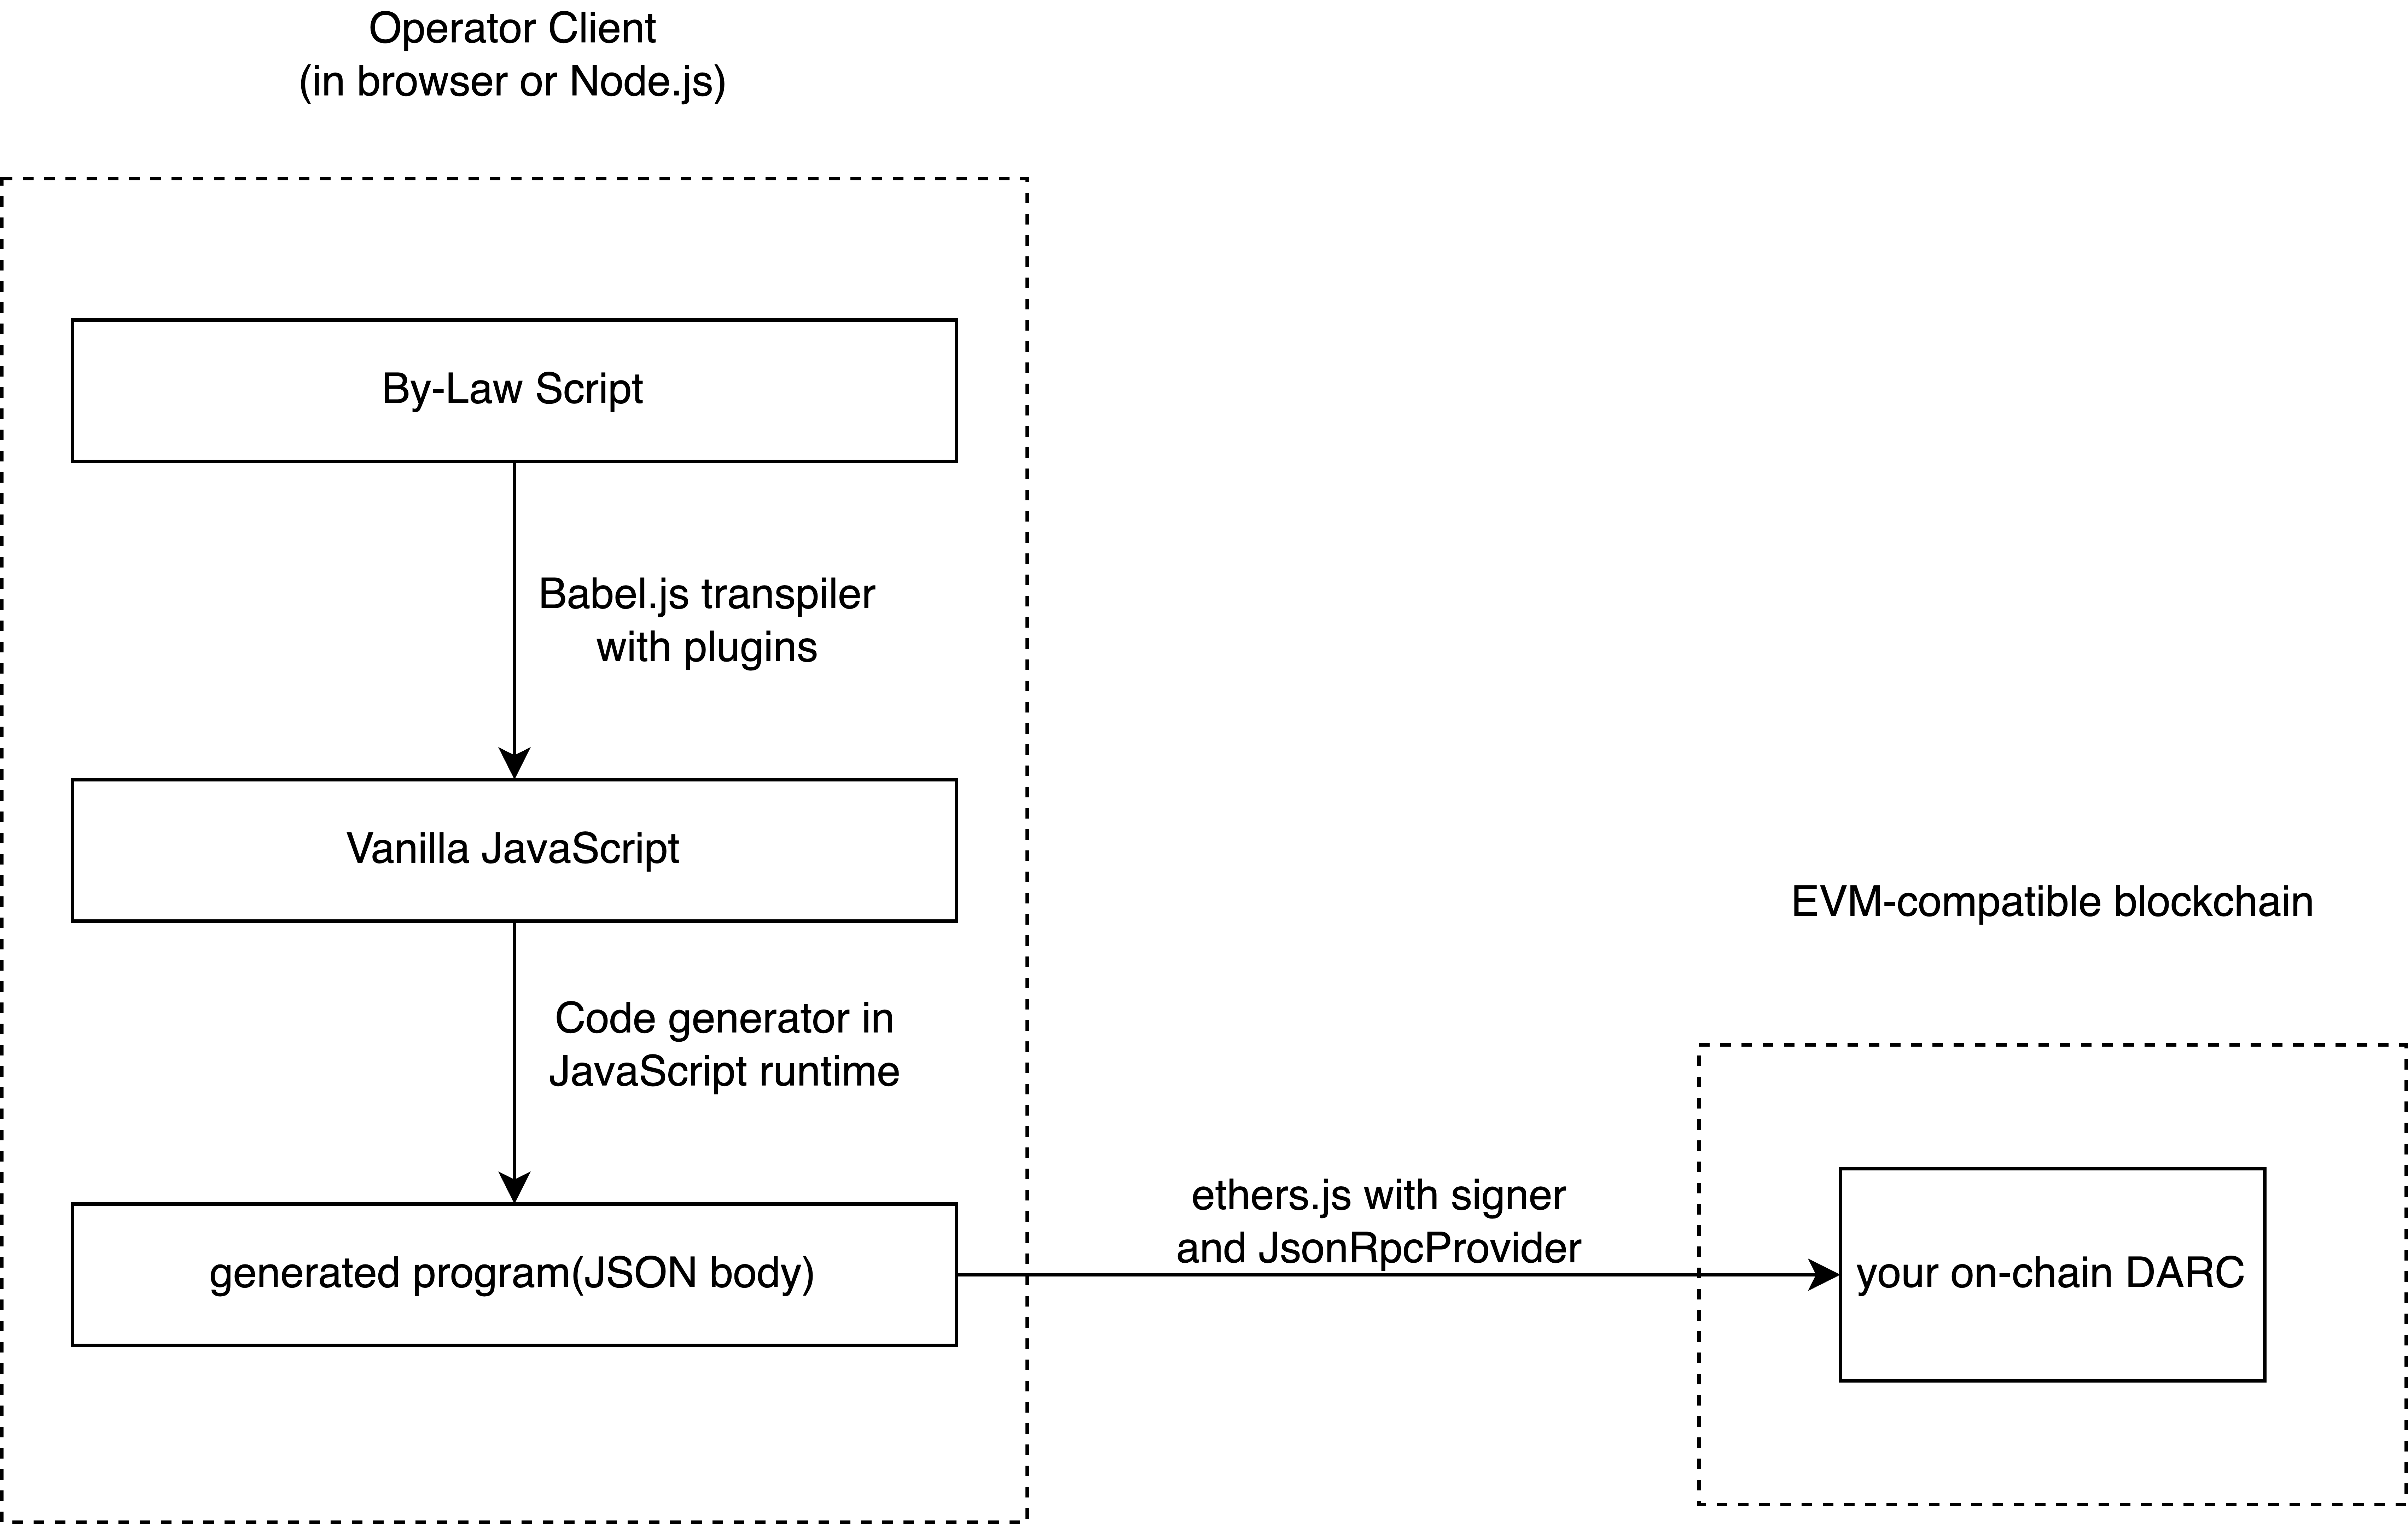
\includegraphics[width=1\linewidth]{by-law.drawio.large.png}
\caption{\label{fig:byLaw}The process of compiling and executing By-law Script}
\end{figure}


\subsection{Transpiler}

After a user runs the By-law Script, the first step in the transpilation process involves converting the By-law Script into vanilla JavaScript. This initial transformation employs Babel.js for front-end syntax analysis and utilizes an operator overloading plugin to generate the resulting vanilla JavaScript code on the back end.

The primary significance of using the operator overloading plugin lies in its ability to transpile the syntax of logical operators within condition nodes designed by the user. Users create plugins to logically connect and describe various condition expressions using logical operators. When these plugins are transpiled with the operator overloading feature, each condition within a plugin is transformed into a tree-like structure expressed as an object constructed using pure functions and parameters.

Furthermore, the transpiler also supports other advanced ECMAScript syntax and syntactic sugar, making it convenient for users to work with.

\subsection{Code Generator}

Once a user has successfully generated vanilla JavaScript from the transpilation of By-law Script, it can be executed within a JavaScript runtime environment, whether it's in Node.js or a web browser.

The user-generated transpiled vanilla JavaScript code includes one or more operation command functions, each comprising opcodes and their corresponding parameters. Upon execution, each of these operation segments is stored in an array, ultimately forming a program object. Subsequently, the code generator leverages this program object to create a complete program JSON body, adhering to the DARC ABI entrance specifications.

Once the program JSON body has been successfully generated, users can utilize ethers.js to send this program body, following the ABI, to the DARC protocol on an EVM-compatible blockchain. This process ensures that the program is executed in its entirety within the DARC.

\begin{figure}
\centering
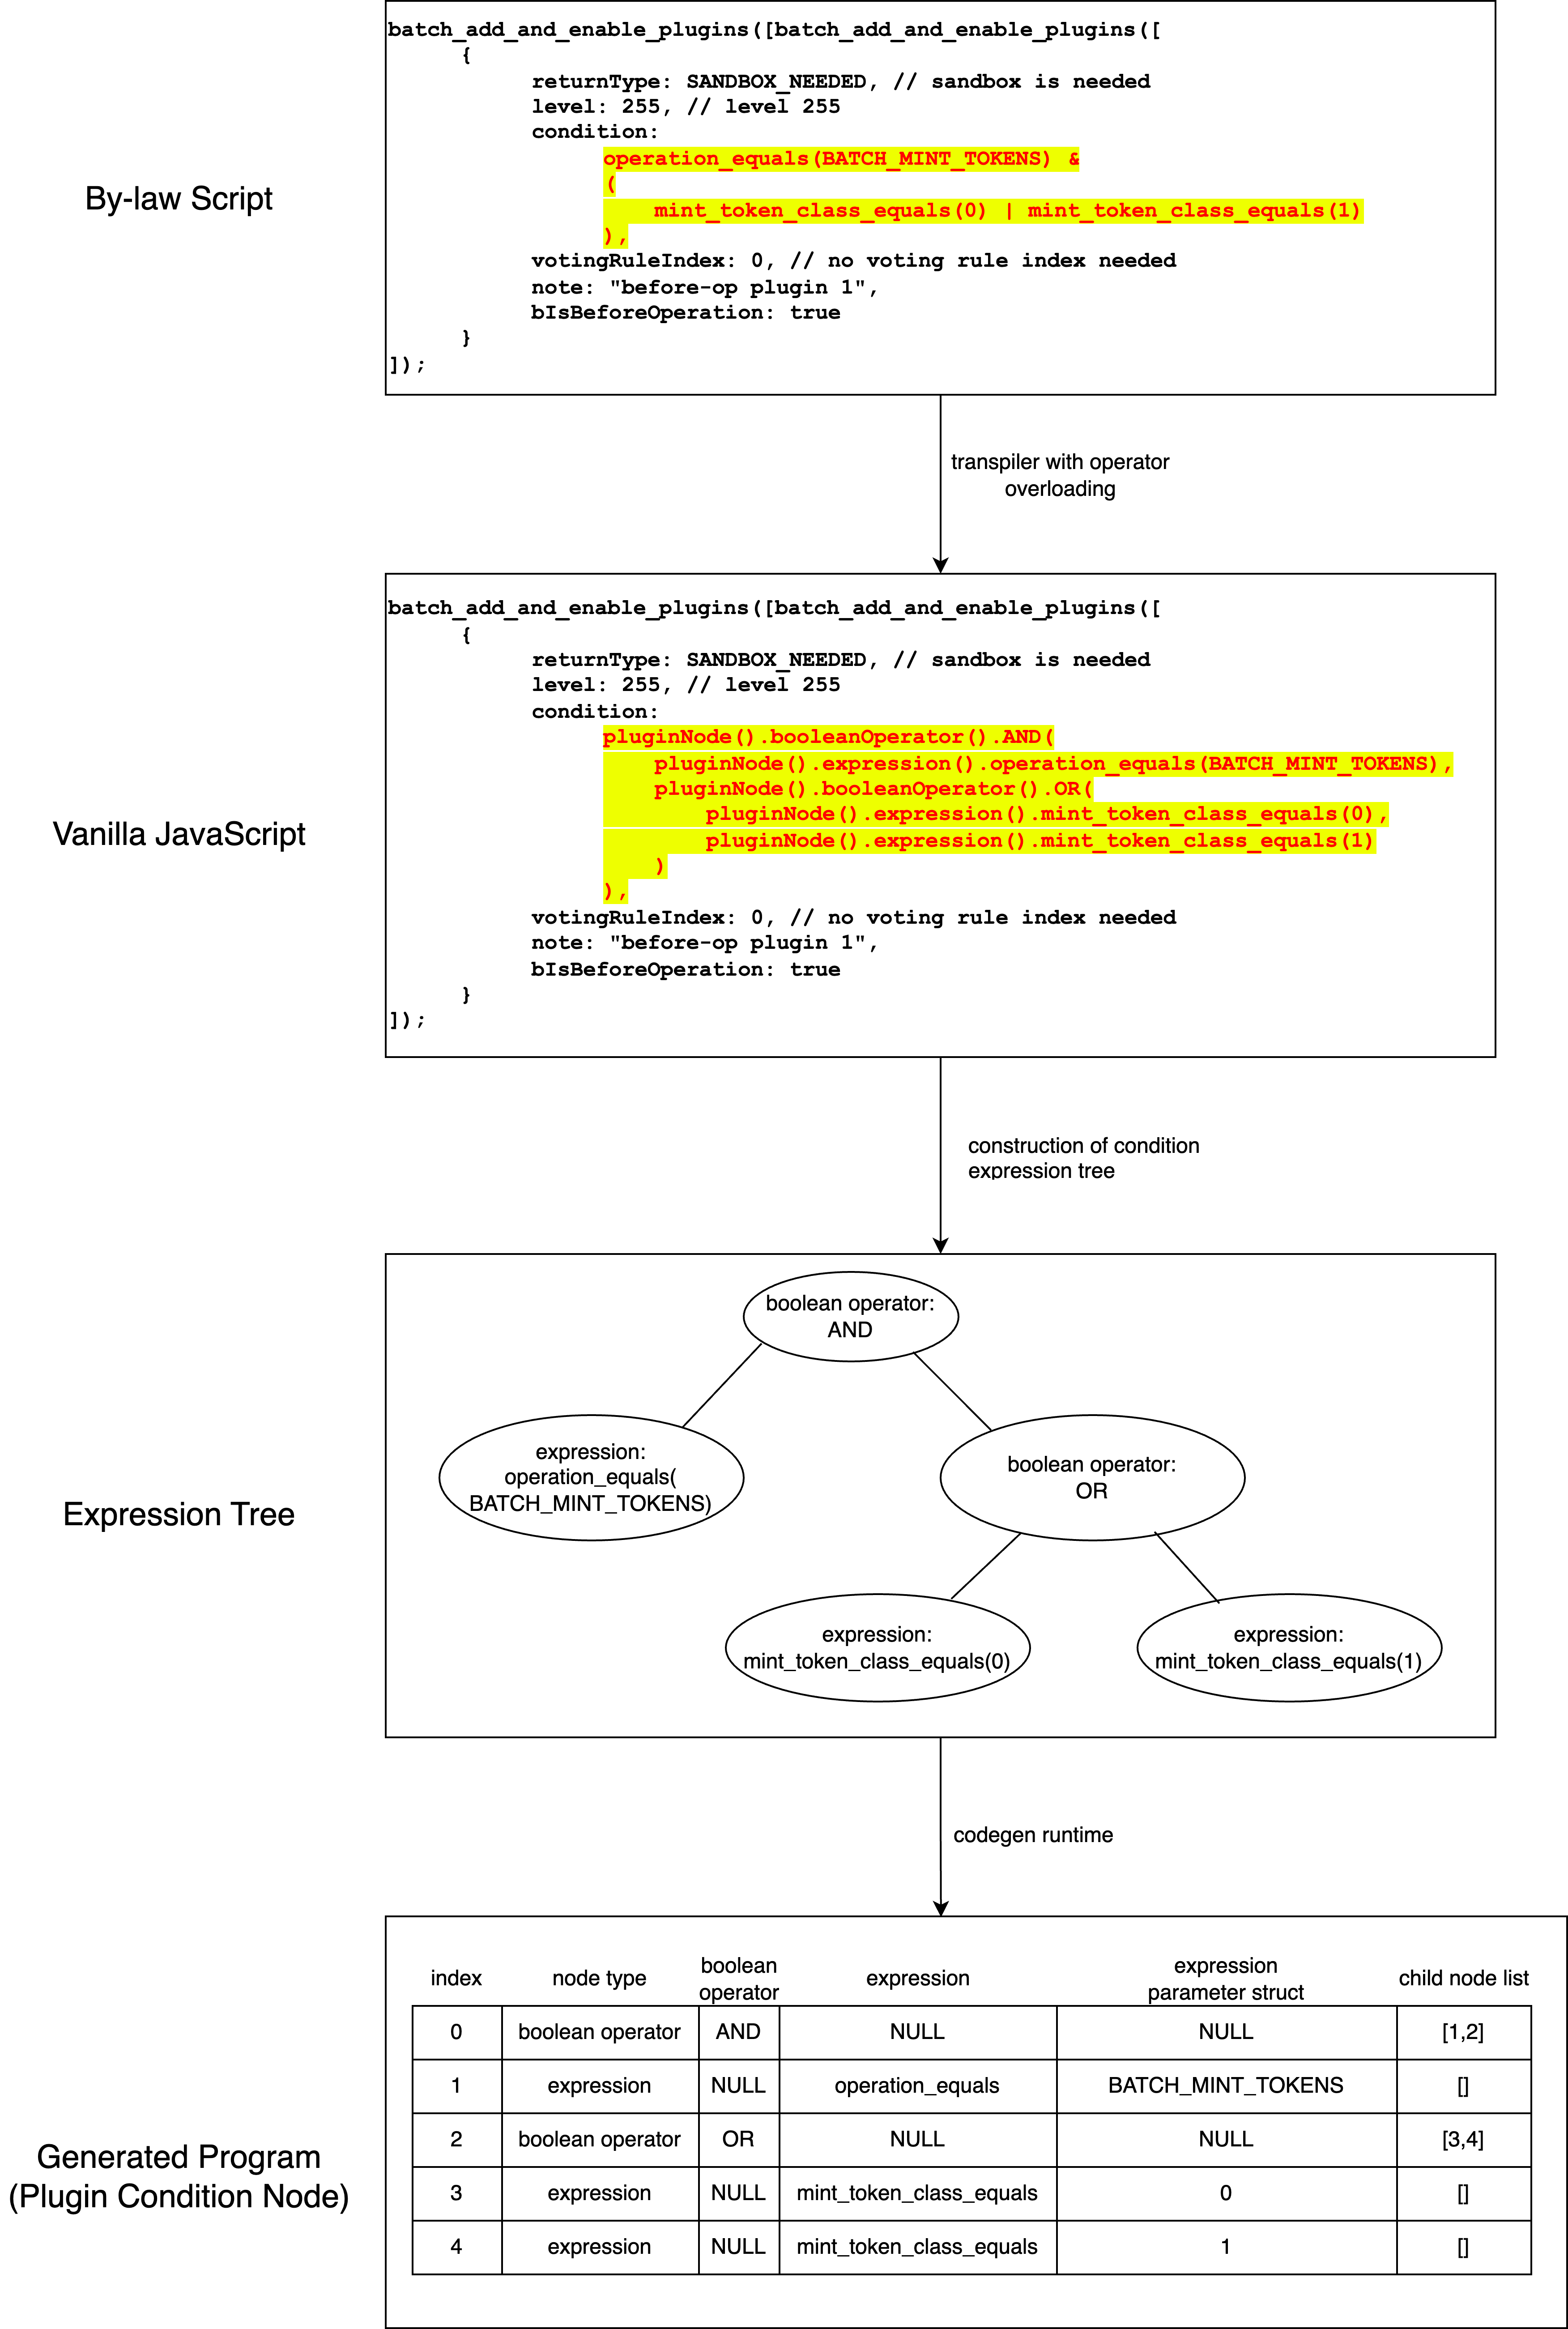
\includegraphics[width=1\linewidth]{by-law-script-process.drawio.png}
\caption{\label{fig:by-law-plugin}Transpiling and Code Generation for Plugins}
\end{figure}

Figure \ref{fig:by-law-plugin} illustrates a complete compilation process. The entire By-law Script toolchain first parses the By-law Script into an expression tree, transpiles it into vanilla JavaScript, and then, within the JavaScript runtime, the code generator of vanilla JavaScript produces a condition node array for plugins in a DARC Program. 





\begin{verbatim}
transfer
\end{verbatim}

\end{document}